
% 和文概要
\begin{abstract}
JavaScriptとAndroid NFCを用いて、実世界GUIを実現するためのフレームワークGoldFishを実装した。GoldFishを使うことで、Androidで実世界の物に触れると触れた対象や使用者、状況によって様々なユーザインタフェースを表示させ、操作できるアプリケーションが簡単に作成できる。
\end{abstract}

% 英文概要
\begin{eabstract}
English abstract.
\end{eabstract}

\maketitle

% 本文ここから
\section{実世界GUI}\label{sec:Introduction}
本研究の目的は、実世界GUI\cite{実世界GUI}を日常的に使えるようにする事である。実世界GUIは、コンピュータのグラフィカルユーザインタフェース(GUI)に似たしくみを実世界で使うという概念である。

塚田らのUbi-Finger\cite{Ubi-Finger}は、対象を指さす事で選択し、ジェスチャーで操作するための手袋型装置を開発した。また暦本は複数のコンピュータ間でマウスのドラッグアンドドロップの様にデータをやりとりする手法\cite{pick-and-drop}を提案した。椎尾らは、マウスとバーコードリーダーを一体化させることであらゆる物に対してマウスで操作できるようにした。\cite{field-mouse}

GUIには、コンピュータの画面上にゴミ箱や窓などの現実世界のメタファーを提示してユーザーに理解しやすくしている部分と、データを扱うためにドロップダウンメニューやスクロールバーなどのディスプレイならではの新しいユーザインタフェースが組み合わさってできている。我々の生活にはたくさんのコンピュータが埋め込まれているが、電子錠つきの自動ドアをキーパッドで操作して開けていたり、ラップトップPCから目の前にあるプリンターに印刷させるのに画面上でプリンタの名前を指定して送信したりと、操作と効果の対応がわかりにくかったり、効率が悪かったりする事がある。そうではなくむしろ、実世界でもGUIのようにメタファーによるインタフェースとデータ操作用インタフェースが混在している方が使い勝手が良いのではないかと考えた。

既存の実世界GUIの研究から、1.対象の指定 2.ジェスチャーやGUIによる操作 3.ユーザーの判別 4.状況の判別 5.他のシステムとの通信が重要であると考えられる。これらを簡単に利用でき、また日常的に使えるような仕組みを作ることが本研究の目的である。


\section{GoldFish}
GoldFishは実世界GUIを実装するためのフレームワークである。Android NFCを使い、実世界の様々な場所に貼ったNFCタグ(RFIDタグ)を読む事でそれぞれ個別のアプリケーションを起動させる事ができる。GoldFish上でのアプリケーションは通常のAndroidアプリケーションの様にJavaとXMLで実装して個々の端末にインストールするのではなく、JavaScriptとHTMLで実装してWeb上に公開し、GoldFishのWebサイトにそのURLとNFCタグの組み合わせを登録する事で各Android端末から呼び出される。プログラミングは初心者には敷居が高く、ましてや実世界の他の機器と連動したプログラムを書く事などは初心者には難しいが、GoldFishを使ったところプログラミング初心者でも半日で研究室の電子扉をジェスチャーで開けるシステムが実装できた。

GoldFishはubif.org\cite{goldfish}で公開されており、ソースコードはgithubで公開されている。\cite{github}


\subsection{GoldFishアプリケーションの例}
GoldFishアプリケーションの例として、実世界コピペを実装した。コンピュータ同士の間でAndroidを用いてコピーアンドペーストができるアプリケーションである。あらかじめコンピュータにNFCタグを貼り付けておき、そこにAndroid端末で触れると金魚掬いの画面が表示される。(図:\ref{fig:copy-paste})この画面でAndroid端末を右に掬うと、現在最前面に表示しているwebページがAndroidにコピーされる。別のコンピュータに触れてから左に流し込むとペーストが行われる。

実世界コピペの実装では、GoldFishアプリケーションは各コンピュータと直接通信していない。GoldFishアプリケーションおよび各コンピュータははインターネット上のクリップボードサーバーと通信する。各コンピュータにはクリップボードクライアントがインストールされていて、それぞれ貼り付けられたNFCタグのIDが実行引数に与えられている。
クリップボードサーバーはサーバーアプリケーションにRubyのSinatraとEventMachineを、データストアにMemCachedを使用して実装した。クリップボードクライアントはwebブラウザ用をGoogle Chrome Extensionで、Mac用アプリケーションをJRubyでそれぞれ実装した。

Android上で動作するGoldFishアプリケーションは、JavaScriptのsetIntervalとgoldfish.accelerometer関数を用いて10ミリ秒毎に加速度センサーを監視する。1G以上の加速度が100ミリ秒以上連続で左右どちらにかかったかによって、Android端末をコピーとペーストどちらにジェスチャ入力したかを判別する。ジェスチャ入力値と端末IDとNFCタグのIDはAjaxでクリップボードサーバーに送信される。goldfish.id関数、goldfish.tag関数がそれぞれ端末IDとNFCタグのID取得に使える。各コンピュータにインストールされたクリップボードクライアントは、cometを用いてクリップボードサーバーから通信があるまで待機する。URLが送られてきた時はwebページを開き、またコピー命令が送られてきた時は現在開いているURLを返信する。

実世界コピペを使うと、これまでコンピュータ間での通信では機器同士が隣にあるにも関わらずデータ送信先の名前を入力したりアイコンをクリックしたりしていた操作を、直接指示でデータ送信できるようになる。他にもプリンターにデータを送信するのではなく、データを手で掴んで投げ込むと印刷されるといった理解しやすいユーザインタフェースが実装できる。

\begin{figure}
  \begin{center}
    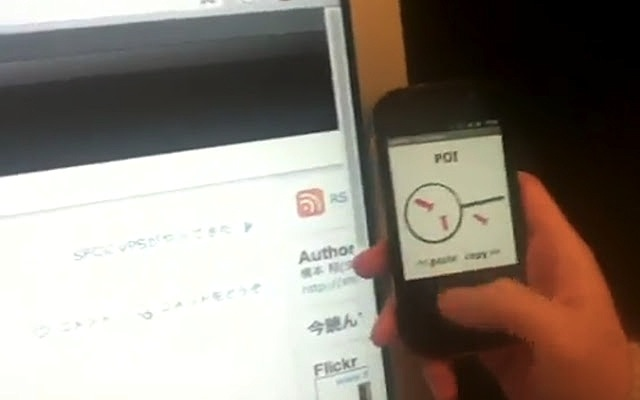
\includegraphics[height=40mm]{img/copy-paste.jpg}
  \end{center}
  \caption{実世界コピペ}
  \label{fig:copy-paste}
\end{figure}


\subsection{GoldFishフレームワークの実装}
GoldFishでは、アプリケーションの実装にAndroidネイティブのJavaではなくJavaScriptを採用している。Javaはプログラム言語自体が複雑で難しく、またセンサーの値を監視しつつ画面を更新しつつ通信も行うなどの並行処理の記述がシンプルに記述できない。JavaScriptはシンプルなプログラム言語で、初心者にもよく薦められている。そして関数がファーストクラスオブジェクトなのでタイマーを用いた並行処理の記述も容易である。

GoldFishはJavaで実装したネイティブアプリに、WebViewコンポーネントでwebページを表示している。WebView内のJavaScriptとAndroidネイティブのJavaが通信する事で、JavaScriptからセンサーなどの機能を呼び出せる。

GoldFishはNFCタグを読んだ際に、あらかじめタグに対して登録されているURLを読み込み、WebViewに表示する。NFCタグはGoldFishのwebサイトで登録できる。(図:\ref{fig:tags})
\begin{figure}
  \begin{center}
    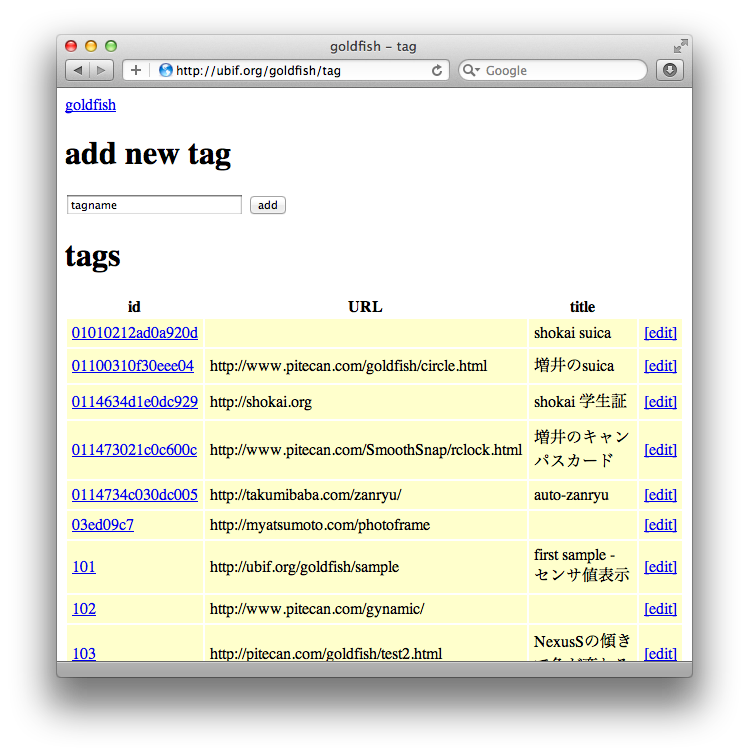
\includegraphics[height=80mm]{img/tags.png}
  \end{center}
  \caption{NFCタグ登録画面 http://ubif.org/goldfish/tag}
  \label{fig:tags}
\end{figure}

\subsection{JavaScriptによるアプリケーションの実装方法}
アプリケーションの実装は、GoldFishのサンプルページ\cite{sample}を見るとわかりやすい。Webページを作成し、goldfish.jsというJavaScriptライブラリを読み込むとAndroidネイティブのセンサーやGoldFish用の様々な機能が使用できる。1章で挙げた実世界GUIの実装に必要な5つの機能は、goldfish.tag関数で操作対象の指定、goldfish.gyroscopeやaccelerometerなどのセンサーによるジェスチャー入力、goldfish.id関数によるユーザーの判別、goldfish.tcpやajaxによるほかのシステムとの通信の組み合わせによって実現できる。


\section{その他のGoldFishアプリケーションの例}
前章の実世界コピペの他にも、いくつかGoldFishを用いた実世界GUIを紹介する。

\subsection{GoldFishドア}
大学の研究室の電子錠ドアをGoldFishで開閉するシステムを実装した。(図:\ref{fig:door})Androidアプリケーション側の実装は、プログラムの基礎は学んだもののあまり書いたことのない大学3年生でも6時間ほどで実装できた。

GoldFishドアは研究室の電子錠ドアに貼ってあるNFCタグに触り、ドアノブをひねるような動きでAndroid端末を回転させると

\begin{figure}
  \begin{center}
    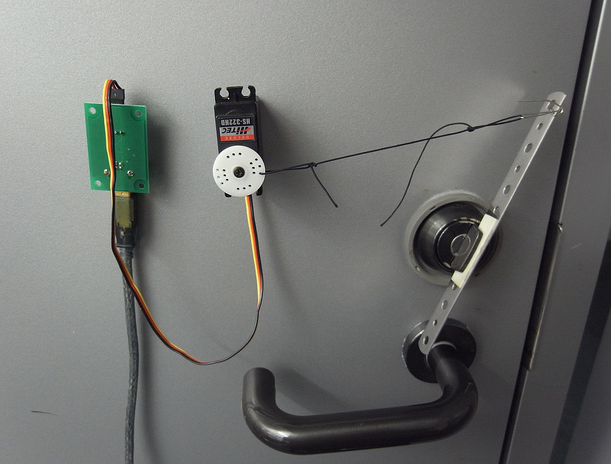
\includegraphics[height=50mm]{img/door.png}
  \end{center}
  \caption{GoldFishドアのしくみ}
  \label{fig:door}
\end{figure}


\subsection{マウス}

\subsection{写真立て}


\section{まとめ}
おまえらGoldFishつかってみろ。いろいろ捗るぞ


\begin{thebibliography}{10}

\bibitem{実世界GUI}
増井俊之. 実世界GUIによる情報家電プログラミング. 情報処理学会ヒューマンインタフェース研究会研究報告 xx-HI-xx, July 2000.

\bibitem{Ubi-Finger}
塚田浩二,安村通晃: Ubi-Finger:モバイル指向ジェスチャ入力デバイスの研究, 情報処理学会論文誌, Vol.43, No.12, pp.3675-3684 (2002)

\bibitem{pick-and-drop}
Jun Rekimoto, Pick-and-Drop: A Direct Manipulation Technique for Multiple Computer Environments, Proceedings of UIST'97, pp. 31-39, 1997.

\bibitem{field-mouse}
椎尾一郎, 増井俊之, 福地健太郎. FieldMouseによる実世界指向インタフェース. コンピュータソフトウェア, Vol.18, No.1, pp. 28-38, January 2001.

\bibitem{github}
GoldFishソースコード. https://github.com/shokai/goldfish

\bibitem{goldfish}
GoldFish. http://ubif.org

\bibitem{sample}
GoldFish App Sample. http://ubif.org/goldfish/sample

\end{thebibliography}

